\documentclass[%
reprint,
amsmath,amssymb,
aps,
]{revtex4-1}
\usepackage{graphicx}% Include figure files
\usepackage{dcolumn}% Align table columns on decimal point
\usepackage{bm}% bold math
\usepackage[utf8]{inputenc}
\usepackage{listings}
\usepackage{amsmath}

\makeatletter
\newcommand*{\rom}[1]{\expandafter\@slowromancap\romannumeral #1@}
\makeatother

\begin{document}
\title{Something}
\author{Torstein S. Ølberg, Ada M. Veddegjerde and Oline A. Ranum}
\affiliation{%
 Universitetet i Oslo \\ Institutt for fysikk\\
 olinear@student.matnat.uio.no : torsteol@student.matnat.uio.no
}
\date{\today}


\begin{abstract}
	The following experiment was undertaken as a mean to explore the different methods of solving a differential equation. We derive the discretized version of the linear one dimentional Poisson equation, implement the Thomas algorithm to write it on a matrix form, specialises this for a tridiagonal matrix, and then rewrite it on a LU decompositional form. What we find is that the difference in relative error is small, but the normal matrix solution and special solution take less time and less memory.

\end{abstract}
\maketitle

\section*{Introduction}

A core feature of the C++ language is the ability to dynamically allocate memory for objects. This is important, ass lagre programs may require very lage lists of numbers to be saved at the same time. If this is not taken into account when writing a program, is may result in unnecessarily slow processes that could, in the worst senarioes crash the program.

In this report we will look at the strenght of dynamically allocating memory and different other algorithms for saving both computation time and memory used when computing a simple linear second-order differential equation.

Linear second-order differential equations have many important applications in science. Such as Poisson's equation who is widely applied in the fields of astronomy, heat flow, fluid dynamics, and electromagnetism (Ford, 2014).

Here we will find a solution for the Poisson equation by rewriting it to different forms, such as a tridiagonal matrix form, a special form only available for tridiagonal cases and an LU decomposition. Then we will calculate the amount of operations of each form we use to make our calculations. We will find a relative error for the different algorithms, and also find the time used for each solution. In the end, we present our results, discuss the positive and negative sides of the different ways we use to solve the linear equation and try to conclude on whether any of the methods are better than the others.

In the Appendix you will find a link to the GitHub repository used to store and track the code for our calculations.
\newpage 

\section*{Theory}
\subsection*{\rom{1}. Discretizing continuous equations}
Linear second-order differential equations such as 
\begin{equation} \label{eq1}
\frac{d^2y}{dx^2}+k^2(x)y = f(x)
\end{equation}
where $f$ is the inhomogeneous term and $k^2$ is a real function, does not always have a known solution. To solve such equations we sometimes have to preform a discretization, and do a numerical computation. For instance, in the case of the Poissons equation who normally reads
\begin{equation*}
\nabla^2 \Phi = -4\pi \rho (\mathbf{r}).
\end{equation*}
we can let $\phi\rightarrow u$ and 
$r\rightarrow x$ and reduce to one dimension so that we have 
\begin{equation}
\label{eq2}
-u''(x) = f(x)
\end{equation}
$u''(x)$ can then often be approximated by the typical Taylor expansion formula
\begin{equation} \label{eq3}
-\frac{v_{i+1}+v_{i-1}-2v_i}{h^2} = f_i  \hspace{0.5cm} \mathrm{for} \hspace{0.1cm} i=1,\dots, n,
\end{equation}
When applying Dirichlet boundary conditions, that is $u(0) = u(1) = 0$, to such systems they are often solvable by rewriting them as a linear set of equations on the form of 
\begin{equation} \label{eq4}
\mathbf{A}\mathbf{v} = \tilde{\mathbf{b}},
\end{equation}
In this paper we will solve such a system where the source term f(x) will be 
\begin{equation} \label{eq5} 
f(x) = 100e^{-10x}
\end{equation}
This yields a closed form solution to equation \ref{eq2} of
\begin{equation} \label{eq6}
	u(x) = 1-(1-e^{-10})x-e^{-10x}
	\end{equation}
	
	\subsection*{\rom{2}. The Thomas algorithm}
	Systems that can be reduced to the form of equation \ref{eq4} where $\bf{A}$ is tridiagonal can be solved by the Thomas algorithm. A simple method consisting of one forward and one backward substitution procedure in order to yield a diagonal matrix with a unique solution. The Thomas algorithm is described by Martin and Boyd (Martin and Boyd, 2010) as method more efficient than the typical Gaussian elimination method. While the number of floating point operations to preform a Gaussian elimination goes like $\mathcal{O}(n^3)$, the Thomas algorithm solves the system in $\mathcal{O}(n)$ operations. The algorithm reduces the tridiagonal system of linear equations to four vectors of size n, and uses a series of elementary row operations to yield a unique solution. For a linear system such as equation \ref{eq4} a row multiplying matrix $\bf{S}$ are applied to eliminate the superdiagonal elements
	\begin{equation*}
	\bf{SAx} = \bf{Sb}
	\end{equation*}
	If $\bf{SA}$ is easier to invert that just $\bf{A}$ then $\vec{x}$ will be easier to obtain. The algorithm takes the foundation of the Gaussian-Jordan elimination with elementary multiplying matrices applied to both sides of the equation. In the end the left side is transformed to an diagonal matrix. 
	
	\subsection*{\rom{3}. Relative error}
	\noindent The relative error of a dataset $\{v_i\}$ and $\{u_i\}$ is given by
	\begin{equation} \label{eq7}
	\epsilon_i = \textnormal{log}_{10} \left( \left\lvert \dfrac{v_i-u_i}{u_i} \right\lvert \right)
\end{equation}

\subsection*{\rom{4}. LU decomposition}
\noindent A lower-upper-decomposition consists of rewriting a matrix $\bf{A}$ into a lower (l) and a upper (u) triangular matrix. The general algorithm for such a decomposition is given by 
\begin{align*}
u_{ii} =& a_{ii} - \sum_{k = 1}^{i-1} l_{ik} u_{ik}  \\
u_{1j} =& a_{1j} \\
l_{ij} =& \left( a_{ij}- \sum_{k = 1}^{J-1} l_{ik} u_{ik} \right) / u_{jj} \textnormal{   for } i > j
\end{align*} 

\noindent When the matrix is decomposed so that 
\begin{equation}
A\vec{x} = LU\vec{x} = b
\end{equation}
one can solve the system by the two following equations. 
\begin{equation} \label{eq8}
\hat{L} (\hat{U}\vec{x}) = \hat{L}\vec{y} = \vec{b}
\end{equation}
We solve for y, then we solve 
\begin{equation} \label{eq9}
\hat{U\vec{x}} = \vec{y}
\end{equation}
To find $\vec{x}$.






\section*{Method}
\subsection*{\rom{1}. Discretizing the system}
\noindent In this paper we will solve equation \ref{eq2} which Dirichlet boundary conditions by rewriting it as a set of linear equations with the restraints
\begin{equation*} 
-u''(x) = f(x), \hspace{0.5cm} x\in(0,1), \hspace{0.5cm} u(0) = u(1) = 0
\end{equation*}
We define the discretized approximation to  $u$ as $v_i$  with 
grid points $x_i=ih$   in the interval from $x_0=0$ to $x_{n+1}=1$.
The step length is defined as $h=1/(n+1)$, so that the boundery conditions give $v_0 = v_{n+1} = 0$.
We  approximate the second derivative of $u$ with equation \ref{eq3} where $f_i=f(x_i)$. Since we have discretized the problem, it is here possible to rewrite equation \ref{eq2} as a linear set of equations on the form of equation \ref{eq4}. To see that this is the case, and to find $\bf{A}$ and $\tilde{\mathbf{b}}$, we first look at the equation for a single point $v_i$ and multiply both sides of sample from equation \ref{eq3} with $h^2$
\begin{equation*}
- v_{i+1} - v_{i-1} + 2v_i = h^2f_i
\end{equation*}
Looking at the left hand side it becomes clear that sum can be rewritten into a dot product between two vectors 
\begin{equation*}
\begin{bmatrix}
-1 & 2 &-1
\end{bmatrix}
\begin{bmatrix}
v_{i-1} \\ v_i \\ v_{i+1} 
\end{bmatrix} = h^2f_i
\end{equation*}
If the equation then is extended to a complete format solving for all $v_i$ simultaneously, we set up the full vector $\bf{v}$ and $\bf{f}$ ranging from \textit{i = 1,...,n} (excluding the known boundaries $v_0 = v_{n+1}$)
\begin{equation*}
\begin{bmatrix}
2 & -1 & 0 & \dots  & \dots & 0 \\
-1 & 2 & -1 & 0 & \dots & \dots \\
0 & -1 & 2 & -1 & 0 & \dots \\
& \dots & \dots & \dots & \dots & \dots \\
0 & \dots &  & -1 & 2 & -1 \\
0 & \dots &  & 0 & -1 & 2
\end{bmatrix}
\begin{bmatrix}
v_1 \\ 
v_2 \\
v_3 \\  
\vdots \\
v_{n-1} \\ 
v_{n}
\end{bmatrix}
= h^2	
\begin{bmatrix}
f_1 \\
f_2 \\ 
f_3 \\ 
\vdots \\
f_{n-1} \\ 
f_n
\end{bmatrix} 
\end{equation*} 
where we recognize that $\tilde{\mathbf{b}} = h^2\bf{f}$ and $\bf{A}$ is the  $n \times n$ tridiagonal matrix. The source term is defined as in equation \ref{eq5}.

\subsection*{\rom{2}. Implementing the Thomas algorithm}
\noindent As matrix $\bf{A}$ is a tridiagonal matrix
this system is solvable by the Thomas algorithm as described in the theory section. In this section we will derive a numerical solution that we will compare to the closed form solution presented in equation \ref{eq6}.  First we will develop a general procedure based on the Thomas algorithm which do not assume a specific form of the elements in A. The algorithm is implement through C++, and the code in its entirety is available in Appendix A. 

\subsection{A general algorithm for solving tridiagonal matrices}
\noindent The general linear equation for a tridiagonal matrix reads
\[
\mathbf{A} = \begin{bmatrix}
b_1& c_1 & 0 &\dots   & \dots &\dots \\
a_1 & b_2 & c_2 &\dots &\dots &\dots \\
& a_2 & b_3 & c_3 & \dots & \dots \\
& \dots   & \dots &\dots   &\dots & \dots \\
&   &  &a_{n-2}  &b_{n-1}& c_{n-1} \\
&    &  &   &a_{n-1} & b_n \\
\end{bmatrix}\begin{bmatrix}
v_1\\
v_2\\
\dots \\
\dots  \\
\dots \\
v_n\\
\end{bmatrix}
=\begin{bmatrix}
\tilde{g}_1\\
\tilde{g}_2\\
\dots \\
\dots \\
\dots \\
\tilde{g}_n\\
\end{bmatrix}.
\]

\noindent This equation can be solved using Gaussian elimination over the extended matrix. The lower off-diagonal elements can be removed using a forward substitution, by iteratively subtracting the former row from the one below. When implementing the algorithm we formulate the matrix as three pointer-based arrays. One array for the diagonal elements of length N, and two for the lower- and upper off-diagonal elements of length N-1. We also define a pointer to store the altered values for the diagonal elements $\{\tilde{b}_i\}$ and the the right hand side off the equation $\{\tilde{g}_i \}$. No subtraction is preformed on the first row, and therefore it remains unchanged throughout the forward substitution so that $\tilde{b}_1 = b_1 $. All other diagonal elements are altered by the process when $\dfrac{a_{i-1}}{b_{i-1}}\cdot c_{i-1}$ is subtracted from the \textit{i}-th row.  

\subsubsection{Forward substitution}
\noindent The general algorithm for this forward substitution is

\begin{lstlisting}[basicstyle=\ttfamily]
for i =  2:n-1
	b~ [i] = b[i] \
	- a[i-1]*c[i-1]/b~[i-1]
	g~ [i] = g[i] \
	- g~[i-1]*a[i-1]/b~[i-1]             
end for
\end{lstlisting} 


\subsubsection{Backward substitution}
\noindent The backward substitution algorithm removes all upper off-diagonal elements $\{c_i\}$. This is a two step process, first a subtraction yielding a diagonal matrix with a unique solution and once again altering $\{\tilde{g}_i\} \rightarrow \{\tilde{\tilde{g}}_i\}$. Then one could calculate every component of the $\{v_i\}$ as $v_i = \tilde{g}/\tilde{b}_i$. Given that we do not need to keep track of $\{c_i\} = 0$, we instead save a couple of floating point operations and one memory storage operation by calculating $\{u_i\}$ directly. The backward substitution looks like

\begin{lstlisting}[basicstyle=\ttfamily]
u [N-1] = g~[N-1]/d~[N-1]
for i =  N-2:1
	u [i] = \
	(g~[i] - c[i]*u[i+1])/b~[i]             
end for
\end{lstlisting} 

\subsection*{\rom{3}. Specialized version}
\noindent If we exploit that the matrix has identical elements along the diagonal and identical (but different) values for the non-diagonal elements it is possible to reduce the number of floating point operations necessary so solve equation \ref{eq4}.  The special case algorithm does not need to keep track off all identical elements. As well, the algorithm can be reduced even futher by pre-calculating $\{\tilde{b}_i\}$. Looking at the first few itterations of $\tilde{b}_i$ we see that:
\begin{equation}
\begin{matrix}
b_1 = 2 \\
\vspace{1mm}
b_2 = 2 - \dfrac{1}{2} = \dfrac{3}{2} \\
b_3 = 2 - \dfrac{3}{2} = \dfrac{4}{3} \\
\vdots \\
b_i = \dfrac{i + 1}{i}
\end{matrix}
\nonumber
\end{equation}
Taking this into account the specialized algorithm reads 


\begin{lstlisting}[basicstyle=\ttfamily]
for i =  2:n-1
 g~ [i] = g[i] + g~[i-1]/b~[i-1]             
end for

u [N-1] = g~[N-1]/d~[N-1]
for i =  N-2:1
 u [i] = (g~[i] + u[i+1])/b~[i]             
end for
\end{lstlisting} 

\noindent First we plot both the results with the analytical solution of equation \ref{eq6}. Then we compare the CPU time for the general and specialized algorithm for matrices up to $n = 10^6$ grid points.  

\subsection*{\rom{4}. Computing the relative error}
We compare the relative error as given by equation \ref{eq7} of the specialized algorithm. We try to increase n to $n = 10^7$, and present all results in tables given in the result section. 

\subsection*{\rom{5}. Armadillo LU decomposition}
\noindent In order to make a comparison to a secondary method, we used the armadillo package. We created the function \textit{LU\_arma} that takes N as an argument and creates the N$\times$N tridiagonal matrix. First we apply the inbuilt armadillo LU-function to the matrix, resulting in one upper and one lower trigonal matrix. Then we use the armadillo solve function to solve equation \ref{eq8} and \ref{eq9}. We plot and compare both time and precision of the armadillo solution to our tridiagonal solver. We also test the standard LU decomposition for a matrix of the size $10^5 \times 10^5$. 

In order to make a comparison to a secondary method, we used the armadillo package. We created the function \textit{LU\_arma} that takes N as an argument and creates the N$\times$N tridiagonal matrix. First we apply the inbuilt armadillo LU-function to the matrix, resulting in one upper and one lower trigonal decomposition. Such that A comes on the form of 
\begin{align*}
\hat{A} =& \begin{bmatrix}
b_1& c_1 & 0 &\dots   & \dots &\dots \\
a_1 & b_2 & c_2 &\dots &\dots &\dots \\
& a_2 & b_3 & c_3 & \dots & \dots \\
& \dots & \dots &\dots   &\dots & \dots \\
&   &  &a_{n-2}  & b_{n-1} & c_{n-1} \\
&    &  &   &a_{n-1} & b_n \\
\end{bmatrix} \\
=& \begin{bmatrix}
1& 0 & 0 &\dots   & \dots \\
a'_1 & 1 & 0 & \dots & \dots \\
\dots & a'_2 & 1 & 0 & \dots \\
& \dots   & \dots &\dots & \\
& \dots  & a'_{n-2}  &1& 0 \\
& \dots  &   &a'_{n-1} & b_n \\
\end{bmatrix}
\begin{bmatrix}
b'_1& c'_1 & 0 &\dots   & \dots \\
0 & b'_2 & c'_2 &\dots &\dots  \\
& 0 & b'_3 & c'_3 & \dots \\
& \dots   & \dots &\dots   &\dots \\
& \dots  & 0 & b'_{n-1} & c'_{n-1} \\
& \dots  &   & 0 & b'_n \\
\end{bmatrix} \\
=& \hat{L}\hat{U}
\end{align*} 
Yielding the equation:
\begin{equation}
A\vec{x} = LU\vec{x} = b
\end{equation}
We then apply the armadillo solve function to this equation in two steps 
\begin{equation}
\hat{L} (\hat{U}\vec{x}) = \hat{L}\vec{y} = \vec{b}
\end{equation}
We solve for y, then we solve 
\begin{equation}
\hat{U\vec{x}} = \vec{y}
\end{equation}
To find $\vec{x} = \vec{u}$

\section*{Results}
\noindent The total number of floating point operations for the general algorithm is 9$\times N$ + 1. That is, $6\times N$ from the forward substitution and $3\times N $ from the backward substitution. The last floating point operation comes from setting the initial u[N-1] varriable. The results of the implementation is presented in figure \ref{fig:1}.

Looking next at the specialized algorithm it is evidently more efficient as it is based on $4 \times N + 1$ floating point operations. This becomes clear when comparing the CPU time when running both algorithms on the same number of grid points. The results are presented in figure \ref{tab1}.

\begin{figure}[!h]
	\begin{tabular} {|c|c|c|}
		\hline
		N & Time gen. alg. & Time spec. alg.\\
		\hline
		 &  &\\
		12      & $ 2.0 \cdot 10^{-6} $ & $ 1.0 \cdot 10^{-6}$ \\
		102     & $ 5.0 \cdot 10^{-6} $ & $ 4.0 \cdot 10^{-6} $  \\
		1002    & $ 3.0 \cdot 10^{-5} $ & $ 2.0 \cdot 10^{-5} $ \\ 
		10002   & $ 3.5 \cdot 10^{-4} $ & $ 2.8 \cdot 10^{-4}$ \\
		100002  & $ 3.5 \cdot 10^{-3} $ & $ 2.7 \cdot 10^{-3}$  \\
		1000002 & $ 4.3 \cdot 10^{-2} $ & $ 3.0 \cdot 10^{-2}$  \\
		\hline
	\end{tabular}
	\label{tab1}
	\caption{Time used by each algorithm with an N X N matrix}
\end{figure}

Next, we looked at the effect of increasing N in regards to the relative error

\begin{figure}[!h]
	\begin{tabular} {|c|c|}
		\hline
		$10^N$ &  $\epsilon_{\textnormal{max}}$ \\
		\hline
		& \\ 
		1 & -0.479697\\
		2 & -1.406193\\
		3 & -2.398478\\
		4 & -3.299038\\
		5 & -4.261650\\
		6 & -5.001046\\
		7 & -0.301030\\
		\hline
	\end{tabular}
	\label{tab2}
	\caption{The max error yielded by formula \ref{eq7} for 10$^N$ grid points.}
\end{figure}

Finally, we compared the results of the tridiagonal solver with the result of the LU decomposition code. The results are plotted for N = 10, 100 and 1000 in figure \ref{N10}, \ref{N100} and \ref{N1000}. When comparing the run time between using the LU decomposition and the tridiagonal solver, it is evident that the tridiagonal solver is faster. The results are presented in table \ref{tab1}. When the LU decomposition is applied to a matrix of $10^4 \times 10^4$, it is no longer successful. This is not surprising as the number of floating point operations for a LU decomposition goes like $\mathcal{O}(n^2)$. This means that int the case of $n = 4$, we obtain about 80 Gb of memory that has to be stored for this single program, which is unlikly for your pc to handle.
\newpage

Finally, we compared the results of the tridiagonal solver with the result of the LU decomposition code. The results are plotted for N = 10, 100 and 1000 in figure \ref{N10}, \ref{N100} and \ref{N1000}. When comparing the run time between using the LU decomposition and the tridiagonal solver, it is evident that the tridiagonal solver is faster. The results are presented in figure \ref{tab2}. When the LU decomposition is applied to a matrix of $10^4 \times 10^4$, it is no longer successful. This is not surprising as the number of floating point operations for a LU decomposition goes like $\mathcal{O}(n^2)$.

\begin{figure}[!h]
	\begin{tabular} {|c|c|}
		\hline
		Run &  Time \\
		\hline
		& \\ 
		1 & 0.587788\\
		2 & 0.591515\\
		3 & 0.563352\\
		4 & 0.595983\\
		5 & 0.571318\\
		6 & 0.567898\\
		7 & 0.567745\\
		8 & 0.586931\\
		9 & 0.586375\\
		10& 0.577970\\
		\hline
		& \\ 
		Average & 0.58 $\pm 0.01 $\\
		\hline
	\end{tabular}
	\label{tab2}
	\caption{The 10 time tests runs using the \textit{time.h} package for the LU-decomposition with N = 1000 grid points, and the average $\pm$ the standard deviation of the runs.}
\end{figure}

\section*{Discussion} 
From the reduction in number of FLOPs in the specific solution compared to the general solution, it is clear that the specialised solution, is better in all cases where it is possible to choose it. Taking up less memory and less time. However, it is only available in very specific situations. As for the Lu decomposition method, it is both slower and takes way more memory compared to both of the other algoritems. But from figure \ref{N10}, \ref{N100} and \ref{N1000} we can see that the error compared to the analytical solution is the same as it is in the normal tridiagonal solutions. \\
\textit{Compare the result with the closed-form solution:}\\
By looking at figure \ref{fig:1} it is evident that the tridiagonal solver approaches the analytical solution as the number of grid points increase from N = 10 to N = 1000.

By looking at figure \ref{fig:1} it is evident that the tridiagonal solver approaches the analytical solution as the number of grid points increase from N = 10 to N = 1000. This indicates a minimum threshold for the solver provide useful and sufficient results. The same systematics are present in the LU-decomposition tracks of figure \ref{N10}, \ref{N100} and \ref{N1000}.  \\
\indent When looking at the time it took to run the general and specific algorithms, as well as the standard LU decomposition solver, it is evident that the specific algorithm is the fastest, followed by the general algorithm and then the LU-decomposition solver. This is not at all surprising in regards to the number of floating point operations necessary to preform each procedure. If we assume that the floating point operations are the dominant time consuming element, then the time it takes should be proportional to the number of operations. It then makes sense that the specific algorithm using approximately $4\times N$ floating point operations  should be somewhat lower than the general algorithm using about $9\times N$ operations. The LU decomposition solver is of a highly general format, and is implemented to solve all kinds of dense matrices Thus the number of floating operations goes like $\mathcal{O}(n^3)$ and the time the solver takes should raise somewhat proportional to this. For N = 1000 we see that the LU decomposer is a order of magnitude $10^3$ larger than the specific and the general algorithm, and agrees well with the expectation. \\
We choose to run the timing test on N = 1000 as one should only do time tests on larger \indent values of N. Due to the finite precision in time, there is possibilities that the granularity og the clock are not able to capture the short run times of a smaller N. We do also assume that the memory reading and writing becomes more negligible in relation to larger N values as the floating point operations are significantly more demanding of time than memory operations. \\
\indent Looking then only at the results produced by the Thomas algorithm, we can get a better look at how the relative error is affected by increasing N-values. It is evident that the max error becomes smaller as we increase N up to N = 6. Although, when we go beyond this point the error seems to become larger again. this threshold 

It should also be stated that for all the experiments beyond the timing of the LU-decomposition solver the time, errors and precision was only calculated once. To improve the certainty of this results the tests should have been run many more times. We did not do this due to limited time factors. 
\newpage 
\section*{Conclusion}
\noindent We can conclude that the tridiagonal solver demands at least N = 1000 grid points in order to be successful from these tests. This is then again seen with the LU-decomposition results of figure \ref{N10}, \ref{N100}, \ref{N1000}. For the case of the tridiagonal solver the LU decomposition does not yield a higher quality of results, but takes significantly more time and memory. Thus for the case of a tridiagonal matrix we can conclude that this method successfully are significantly more efficient than the LU-decomposition solver by an order of $10^3$ in time. We also found that by exploiting certain properties of the matrix, in this case the similarity of the matrix elements, we could further increase the efficiency of the matrix. \\
\indent In the case of our $N\times N$ matrix where we have looked primarily at $N=1000$, the results are of limited value as the computer either how takes less than a second to preform the given task. Still the results are of great value, as it states something of the choices made when approaching numerical problems. As N increases, the problem at hand will be more and more demanding. As we saw, the LU decomposition solver was not even capable of taking a matrix of $10^4 \times 10^4$ grid points While the Thomas algorithm let us easily solve the equation with N values up to $10^6$. By selecting a smarter route, we could preform calculations not possible through regular use of the armadillo library. This is important in solving real world problems, as the granularity in real world examples tends to be extremely low for a variety of different experiments. 



\newpage 
\onecolumngrid
\section*{Bibliography}
\noindent $[1]$ W. Ford, Numerical Linear Algebra with Applications, Academic Press 2014, 1st edition.\\ 
$[2]$ Conte, S.D., and deBoor, Elementary Numerical Analysis, McGraw-Hill 1972, New York \\ 
$[3]$ A. Martin and L. Boyd, Variant of the Thomas Algorithm for opposite-bordered tridiagonalsystems of equations, International Journal for Numerical Methods in Biomedical Engineering, 2010, Vol.26, pp.752-759

\section*{Appendix A}
For the code used for calculation our results, visit
\url{https://github.com/OlineRanum/FYS3150_Project_1}


\begin{figure}
	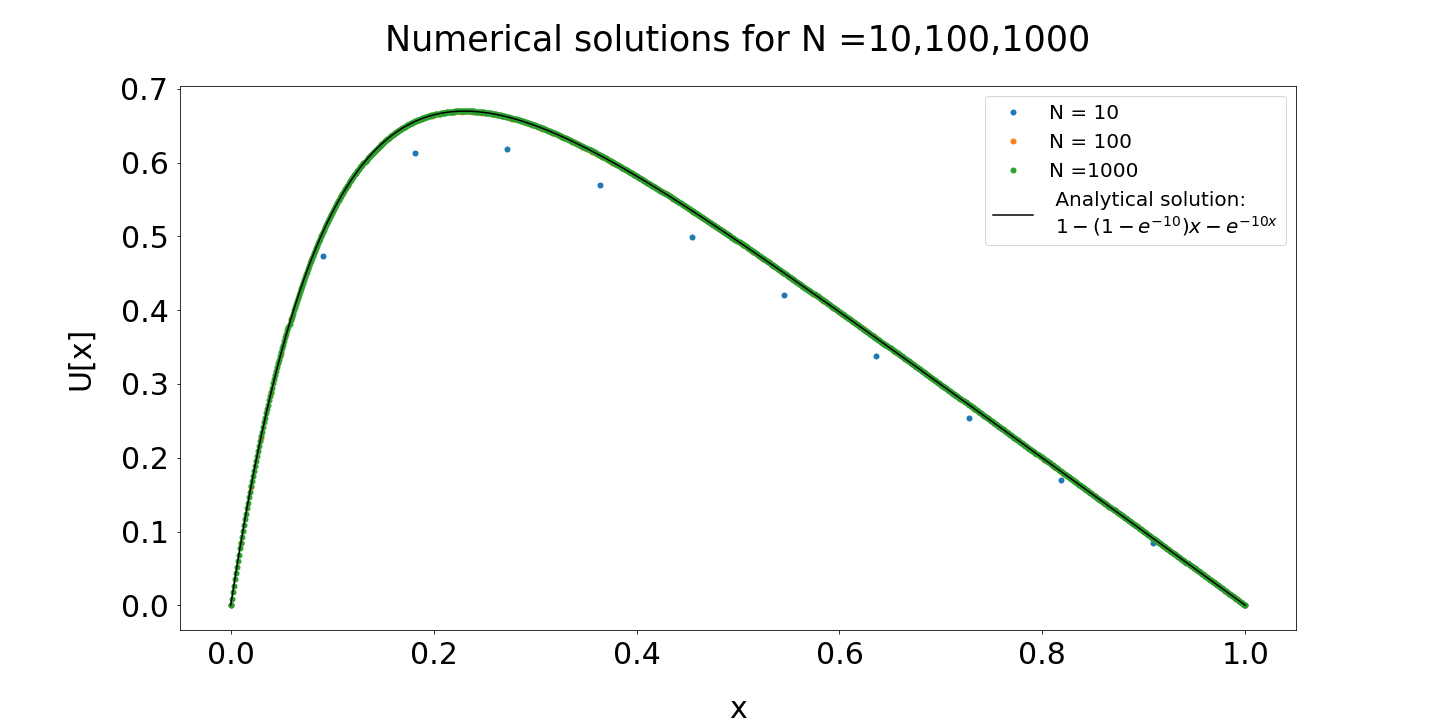
\includegraphics[width=\textwidth]{Numerical_solutions.png}
	\caption{The tridiagonal solver solutions to equation \ref{eq4} for N = 10, 100 and 1000. Plotted alongside the analytical solution of equation \ref{eq6}. }
	\label{fig:1}
\end{figure}

\begin{figure}
	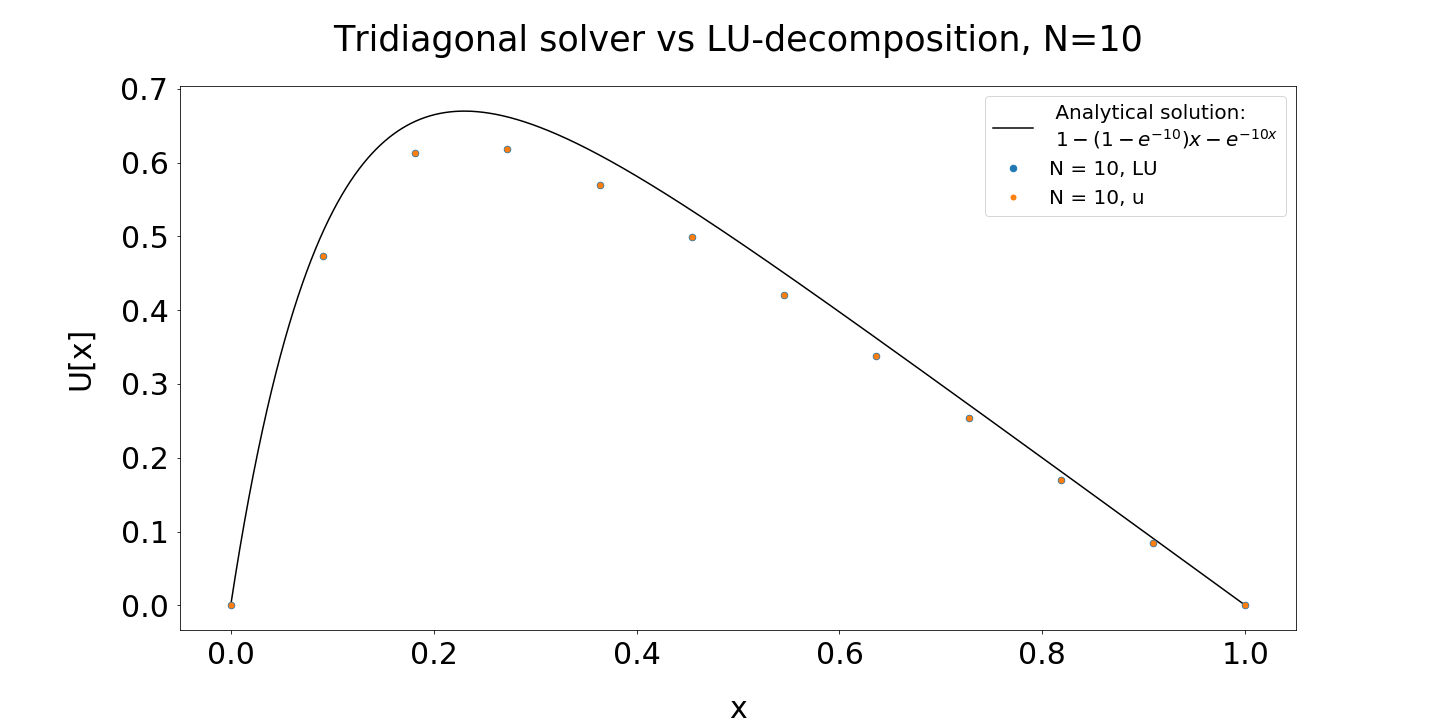
\includegraphics[width=\textwidth]{N_LU_10.png}
	\caption{The solution of the tridiagonal solver vs the LU decomposition solver for a matrix of 10$\times$10 grid points. }
	\label{N10}
\end{figure}

\begin{figure}
	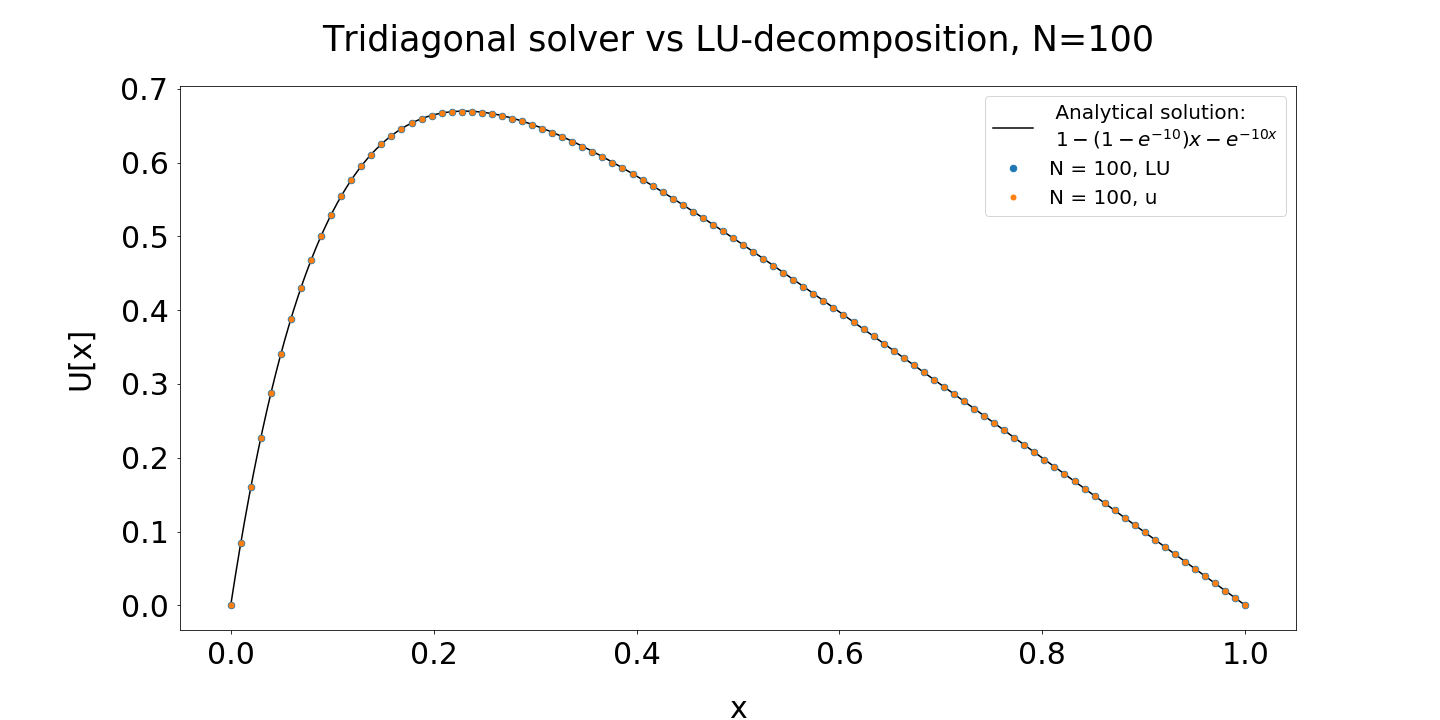
\includegraphics[width=\textwidth]{N_LU_100.png}
	\caption{The solution of the tridiagonal solver vs the LU decomposition solver for a matrix of 100$\times$100 grid points.}
	\label{N100}
\end{figure}

\begin{figure}
	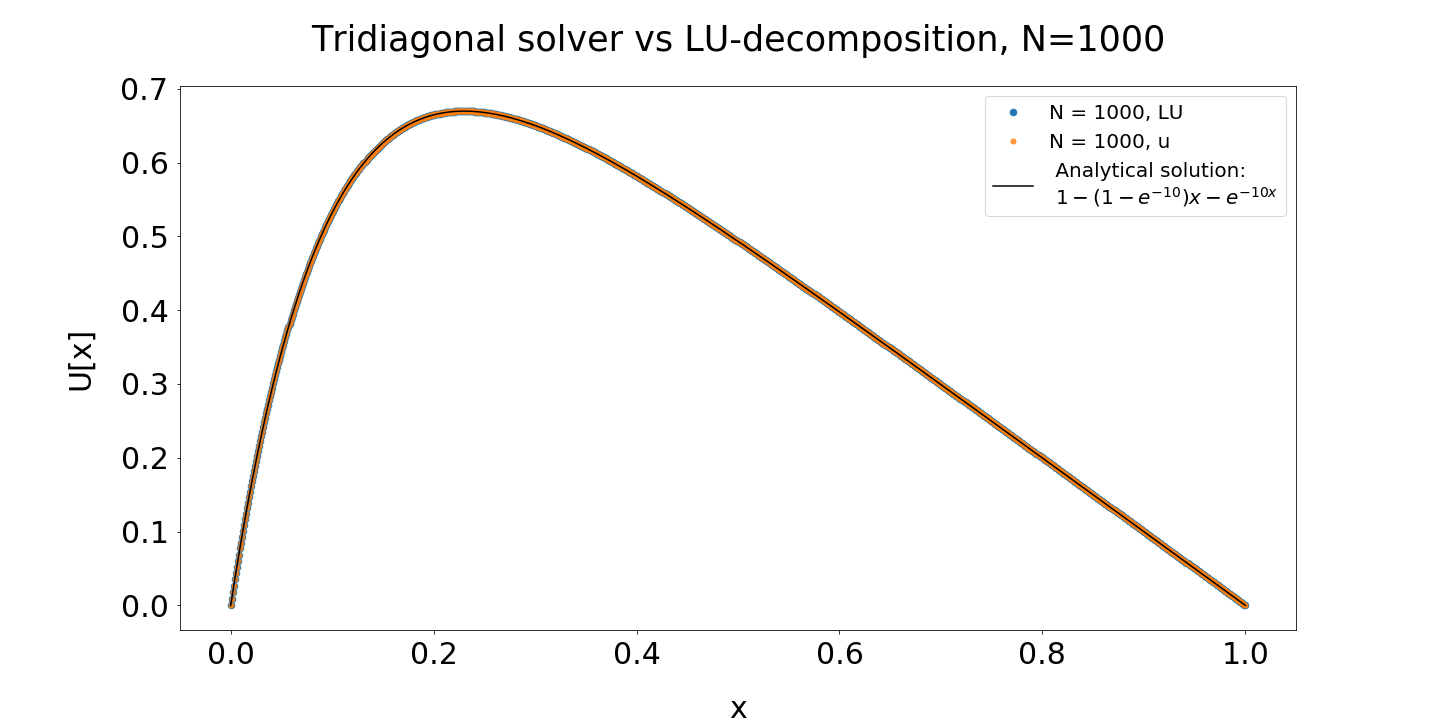
\includegraphics[width=\textwidth]{N_LU_1000.png}
	\caption{The solution of the tridiagonal solver vs the LU decomposition solver for a matrix of 1000$\times$1000 grid points.}
	\label{N1000}
\end{figure}


\end{document}